\section*{Глава 2. Неизотермическая фильтрация флюида к несовершенным скважинам.}
\addcontentsline{toc}{section}{Глава 2. Неизотермическая фильтрация флюида к несовершенным скважинам.}

\setcounter{section}{2}
\setcounter{subsection}{0}
\setcounter{equation}{0}


\subsection{Виды несовершенств}
	В ходе бурения, освоения и эксплуатации скважины различные технологические процессы воздействуют на ОЗП.
	В результате её ФЕС меняются.
	Отличие притока скважины от притока, рассчитанного по формуле Дюпюи учитывают, вводя \textit{скин-фактор} $s$:
\begin{equation}
	\label{dupuit}
	Q = \frac{2\pi k h}{\mu B \left(\ln\displaystyle\frac{r_e}{r_w}+s\right)}
\end{equation}

	Понятие скин-фактора достаточно расплывчато, на него списывают любое отличие от выражения \eqref{dupuit}, зачастую не уточняя чем то или иное дополнительно фильтрационное сопротивление (или даже проводимость) вызвано. Предполагается, что скин-фактор аддитивен. В общем виде можно его представить как \cite{mukerdzhi}:
\begin{equation}
	\label{skin_full}
	s = s_d + s_p + s_{pp} + s_{turb} + s_o + s_s + \cdots,
\end{equation}
	где
\begin{itemize}
\item $s_d$ -- скин эф-т вследствие повреждения породы,
\item $s_p$ -- скин эф-т из-за перфорации,
\item $s_{pp}$ -- скин эф-т вследствие частичного проникновения скважины в пласт,
\item $s_{turb}$ -- скин эф-т вследствие турбуленции или скин, зависящий от темпа отбора,
\item $s_{o}$ -- скин-эффект вследствие наклона скважины,
\item $s_{s}$ -- скин-эффект, возникающий вследствие стимуляции, применения различных МУН.
\end{itemize}
	С формальной точки зрения, каждый из перечисленных выше скин-факторов -- упрощение модели фильтрации и её сведение к случаю радиальной притока. В данной работе будут рассмотрены лишь первые три фактора ($s_d$, $s_p$, $s_{pp}$) из перечисленных, обуславливающие несовершенство скважины, в явной математической поставке, без каких-либо упрощений.

\subsubsection{Повреждение ОЗП}
	В процессе бурения скважины происходит загрязнение ОЗП фильтратом бурового раствора.
	В дальнейшем повреждение ОЗП пожет произойти при проведении геофизических и промысловых исследований, установке и цементированию эксплуатационной колонны, освоении и заканчивании скважины. На Рис. \ref{pic:near_wellbore} представлена типичная структура ОЗП. В ней выделяют внешнюю/внутреннюю фильтрационные корки, зону проникновения фильтрата.
\begin{figure}[H]
	\label{pic:near_wellbore}
	\centerline{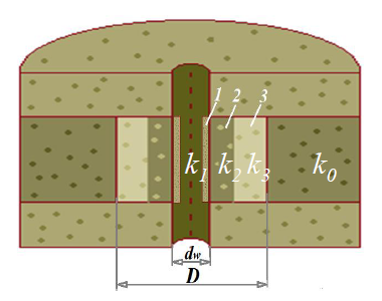
\includegraphics[width=0.6\textwidth]{pic/near-wellbore.png}}
	\caption{Структура ОЗП, образующаяся в результате различных технологических операций. Выделяют:
	\textit{1} -- внешняя фильтрационная корка,
	\textit{2} -- внутренняя корка (зона кольматации), 
	\textit{3} -- зона проникновения фильтрата.}
\end{figure}

	Тем не менее, без особой нужды, при моделировании притока к скважины не рассматривают такую сложную структуру ОЗП. Обычно считают, что вокрук скважины есть кольцевая область с ухудшенной проницаемостью $k_d \leq k$, cм. Рис \ref{pic:near_wellbore_our}.

	При таком подходе скин-фактор $s_d$, отвечающий за повреждение породы, можно найти из выражения:
\begin{equation}
	\label{skin_damage}
	s_d = \left(\frac{k}{k_d}-1\right)\ln\left(\frac{r_d}{r_w}\right).
\end{equation}

\begin{figure}[H]
	\label{pic:near_wellbore_our}
	\centerline{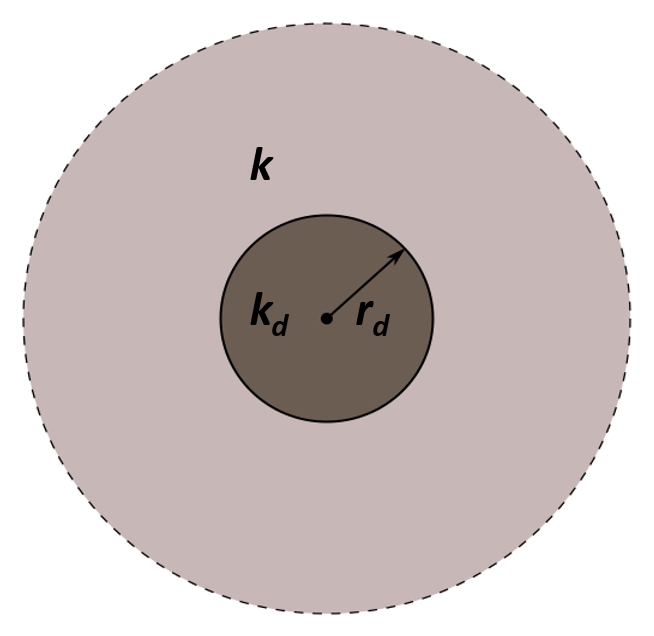
\includegraphics[width=0.4\textwidth]{pic/near-wellbore-our.png}}
	\caption{Рассматриваемая модель ОЗП, обладает ухудшенной проницаемостью $k_d \leq k$.}
\end{figure}

\subsubsection{Перфорация}
	В конструкцию большинства скважин входит обсадная колонна, которая цементируется с внешней стороны.  Для вызова притока в такой схеме исользуется \textit{вторичное вскрытие} продуктивных горизонтов. Одним из наиболее распространённых методов вторичного вскрытия является применение кумулятивных зарядов, которые устанавливают по спирали и спускают на глубину.
Результатом их использования являются перфорационные каналы (ПК), которые прошивают обсадную колонну, цемент и часть ОЗП. На Рис. \ref{pic:tunnels} изображена характерная схема ПК на забое скважины.

	В результате в ОЗП, области с наибольшим градиентом давления в пласте, течение существенно отличается от радиального, т.к приток теперь сосредотачивается у боковых поверхностей каналов.

	Тем не менее, для такого типа перфорации, в \cite{tariq} приведены корреляции скин-фактора $s_p$, в зависимости от длины каналов $L_p$, угла фазировки $\theta$, расстояния по глубине между каналами $h$, радиуса перфорационного отверстия $r_p$, могут быть записаны в следующем виде:
\begin{align}
	\label{tunnels_skin}
	s_p &= s_H + s_V + s_{wb}, \\
	s_H &= \ln\left(\frac{r_w}{r_{we}}\right), \quad r_{we} = 
	\begin{cases}
		\frac{L_p}{4}, &\quad \theta = 0,\\
		\alpha_{\theta}(r_w + L_p), &\quad \theta \neq 0,
	\end{cases}\nonumber\\
	s_V &= 10^a\left(\frac{h}{L_p}\sqrt{\frac{k_{xx}}{k_{zz}}}\right)^{b-1}\left(\frac{r_p}{2h}\left(1+\sqrt{\frac{k_{zz}}{k_{xx}}}\right)\right)^b,\nonumber\\
	s_{wb} &= c_1(\theta)\exp\left(c_2(\theta)\frac{r_w}{L_p+r_w}\right),\nonumber
\end{align}
	где корреляции для величин $\alpha_{\theta}$, $a$, $b$, $c_1$, $c_2$ можно найти непосредственно в \cite{tariq}, $k_{xx}$ и $k_{zz}$ -- проницаемости пласта в вертикальном и горизонтальном направлениях.

\begin{figure}[H]
	\label{pic:tunnels}
	\centerline{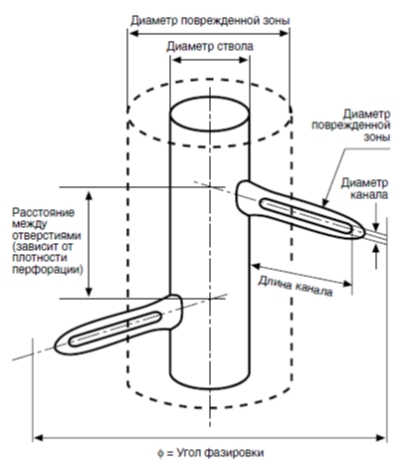
\includegraphics[width=0.6\textwidth]{pic/tunnels.png}}
	\caption{Характерная схема расположения ПК.}
\end{figure}

	Корреляции \eqref{tunnels_skin} найдены также с использованием явного численного расчёта соответствующих постановок. Ниже будет представлено сравнение численного расчёта постановки, проводимого в текущей работе, с каналами с представленными корреляциями.

\subsubsection{Частичное проникновение}
	
	С точки зрения терминологии, представленной например в \cite{basniev}, несовершенства скважины разделяют на два типа: скважина несовершенная по \textit{характеру} и \textit{степени} вскрытия. Характер вскрытия был рассмотрен в двух предыдущих пунктах. Степень вскрытия частично рассмотрена в предыдущем пункте. Однако с методологической точки зрения следует рассмотреть отдельно случай частичного проникновения скважины в пласт, неполного его вскрытия.
В данном примере считается что скважина вскрыта в некотором интервале глубин, не содержащим всю мощность пласта, полностью по всему диаметру.

	Впервые выражение для притока к гидродинамически несовершенной по степени вскрытия скважине получил М. Маскет \cite{masket} методом изображений.
	Затем И.А. Чарный \cite{charniy} получил выражение для дополнительного гидродинамического сопротивления:
\begin{align}
	\label{skin_part_penetr}
	s_{pp} &= \left(\frac{1}{\bar{h}}-1\right)\ln\frac{4h}{r_w}-\frac{\phi(\bar{h})}{2\bar{h}}, \\
	\phi(\bar{h}) &= \ln\frac{\Gamma(0.875\bar{h})\Gamma(0.125\bar{h})}{\Gamma(1-0.875\bar{h})\Gamma(1-0.125\bar{h})},\nonumber
\end{align}
	где $\bar{h} = \displaystyle\frac{b}{h}$ -- доля вскрытой мощности пласта, $\Gamma(n)$ -- гамма-функция Эйлера.

	Отдельным интересным вопросом при расчёте частично перфорированной скважины (как, впрочем, и каналов) является распределение дебита вдоль перфорированной части.


\subsection{Теплоперенос при фильтрации к несовершенной скважине}
	Выше были рассмотрены основные виды несовршенств скважины, рассматрваемые в данной работе, а также представлены приближённые формулы для расчёта дополнительного гидродинамического сопротивления, возникающего в результате данных несовершенств.
	Подобное рассмотрение возможно лишь в однофазном случае, хотя и для случая многофазной фильтрации приводится некая аналитика.
	Рассмотрим влияние этих несовершенств на поведение забойной температуры.

\subsection{Случай совершенной скважины}
	Для начала установим выражение для забойной температуры для притока к совершенной скважине.
	Пренебрегая теплопроводностью запишем уравнение баланса энергии в следующем виде:
